% !TEX root=../master.tex

\chapter{Experimental Apparatus}
\label{chp:experimental_apparatus}

This chapter describes the software and hardware used in the experiments that
are detailed in Chapters~\ref{chp:estimation_paper} and~\ref{chp:control_paper}.

\section{Software}
\subsection {Robot Operating System}
The same C++ algorithm implementations were used both in hardware and simulation
experiments.
This was made possible, in part, due to the use of the Robot Operating System\footnote{Robot Operating System:
\href{www.ros.org}{www.ros.org}} (ROS) as a middleware. ROS provides a way for separate
programs, or nodes, to share information between one another.

A network diagram of the software system can be seen in~\figref{fig:network_diagram}. The estimator and
controller for the UAV were implemented as two separate nodes. 
The estimator node provided the state estimate of the UAV to the controller node.
The controller node computed the desired control action based on the error
between the estimated state and the desired state. This desired control action
was sent to the ROSflight flight control stack~\cite{jackson2016rosflight}
which then actuated either a simulated UAV or the UAV hardware platform.

\begin{figure}[htbp]
  \centering
  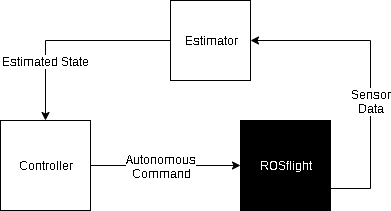
\includegraphics[width=3.5in]{figures/roscopter.png}
  \caption[Software Architecture Network Diagram]{A network diagram of the
  software running during both simulation and hardware experiments.}
%
  \label{fig:network_diagram}
\end{figure}

\subsection {Gazebo}
For simulation experiments, the Gazebo\footnote{Gazebo:
\href{www.gazebosim.org}{www.gazebosim.org}} simulation environment was used with the ROSflight software-in-the-loop
(SIL) simulation.
% This SIL simulation meant that not only the same estimator and controller nodes
% were running in simulation as in hardware, but also the same software from the
% flight controller.
This simulation setup provided for an easier transition from software
experiments to
hardware experiments.

% This simulation setup allowed the
% same estimator and controller implementations to
% be used in the simulation experiments as are used in the hardware experiments,
% making the transition from simulation to hardware less difficult.

\subsection {ROScopter}
The estimator and controller nodes of the ROScopter\footnote{ROScopter:
\href{www.github.com/byu-magicc/roscopter}{www.github.com/byu-magicc/roscopter}}
project were also used during certain points of the simulation and hardware
experiments described in this thesis. In the experiments of the estimator proposed in
Chapter~\ref{chp:estimation_paper}, the ROScopter controller node was used to
close the loop around the produced estimates. In the experiments of the 
controller proposed in Chapter~\ref{chp:control_paper}, the ROScopter estimator node
was used to provide state estimates of the UAV to the controller.

\section{Hardware}
The multirotor UAV used in hardware experiments can be seen
in~\figref{f:drone_pic}. The UAV was built on a DJI Flamewheel 450 frame.
Specific components contained on the UAV are detailed in the following
subsections.

\subsection{Flight Controller}
The multirotor UAV was equipped with an OpenPilot CC3D Revolution 32 bit F4
flight controller as shown in~\figref{fig:f4}. The flight controller ran the
ROSflight firmware which provided an easy interface
for the controller node on the onboard computer to control the UAV.

\begin{figure}[htbp]
  \centering
  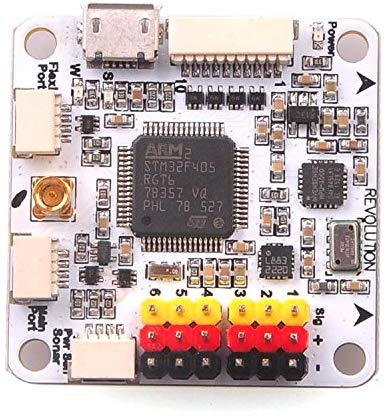
\includegraphics[width=2.5in]{figures/f4.jpg}
  \caption[OpenPilot CC3D Revolution 32 bit F4]{OpenPilot CC3D Revolution 32
    bit F4 flight controller. \\ \hspace{\textwidth} Source:~\cite{openpilotrevo}
}
%
  \label{fig:f4}
\end{figure}

\subsection{Onboard Computer}
The computer onboard the UAV was an NVIDIA Jetson TX2 equipped with an Orbitty
carrier board. This configuration is shown in~\figref{fig:tx2_orbitty}. All
computation was done on the onboard computer during the hardware experiments.

\begin{figure}[h]
  \centering
  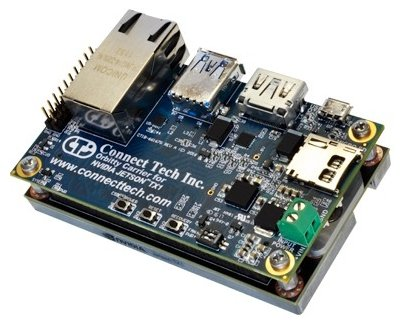
\includegraphics[width=2.5in]{figures/tx2_orbitty.jpg}
  \caption[NVIDIA Jetson TX2 with Orbitty Carrier Board]{NVIDIA Jetson TX2
  with an Orbitty carrier board attached. \\\hspace{\textwidth} Source:~\cite{orbitty}
  }
  \label{fig:tx2_orbitty}
\end{figure}

\subsection{Motion Capture}
Hardware flight experiments were performed in the motion capture room in the
MAGICC Lab at Brigham Young University. This room is equipped with an OptiTrack\footnote{OptiTrack:
\href{www.optitrack.com}{www.optitrack.com}} motion tracking system that
provided high-rate measurements of the position and attitude of the multirotor
UAV during the experiments.

\subsection{Camera}
For the hardware experiments described in Chapter~\ref{chp:estimation_paper},
the multirotor UAV was outfitted with an ELP USB camera with a 2.1 mm lens as
shown in~\figref{fig:camera}. The intrinsic parameters of the sensor were
accurately calibrated using a software package provided by ROS\footnote{ROS
camera\_calibration:
\href{wiki.ros.org/camera_calibration}{wiki.ros.org/camera\_calibration}}.
However, the mounting position and attitude of the camera were only roughly
approximated.

\begin{figure}[h]
  \centering
  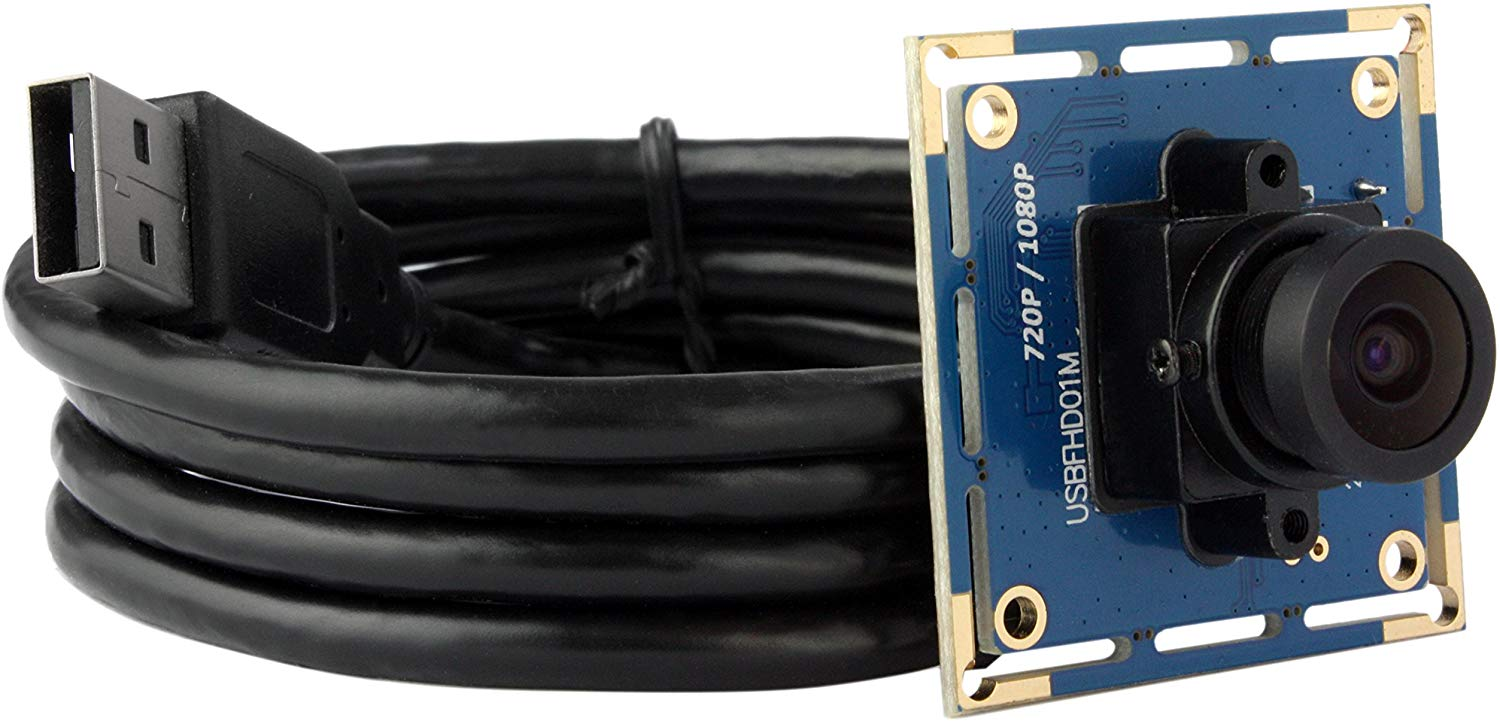
\includegraphics[width=2.5in]{figures/camera.jpg}
  \caption[ELP USB Camera with 2.1 mm Lens]{ELP USB Camera with a 2.1 mm
  lens.

  Source:~\cite{webcam}
}
%
  \label{fig:camera}
\end{figure}

